\chapter{Bevezetés}
\label{chapIntroduction}

A szoftverfejlesztés a mai világunk egyik alapköve. Az informatika világa és a mi hétköznapijaink sem lennének képesek fejlődni a szorgos programozók munkája nélkül. Azonban a szoftver fejlesztés nem egy egyszerű dolog, főleg ha egy komplex programozási feladatra van szükség. Ilyenkor szinte biztosan nem egy ember fogja elkészíteni ezeket a programokat, így a munka érdemi része kevesebb feladatot ró a fejlesztőre viszont számos egyéb feladattal kell szembe néznie.

Ezek a feladatok (ha jól elő vannak készítve) nagyon könnyen vehető akadályok. A csapatban való munka fontos részét alkotja a modern szoftverfejlesztésnek.

A csapatmunkát komoly támogatási háttérrel szükséges ellátni. 
Gondok itt arra, hogy lehetőséget kell adni minden fejlesztő számára, hogy a fejlesztés állapotát nyomon tudják követni és a mások munkáját is könnyen feltudják használni vagy esetenként módosítani tudják azt. 
Fontos az is, hogy 

Szoftver fejlesztés
csapat munka - ugyan olyan formátumú kód - kód felhasználás - dokumentáció
ennke a támogatása
maga a CI fontossága


\section{Motiváció}
\paragraph{}
A Miskolci Egyetem Mérnökinformatikai szakán eltöltött éveim során próbáltam a lehető legtöbb olyan sávot választani a tantervi hálóból ami nem fejlesztéssel hanem üzemeltetéssel foglalkozik. 
A fejlesztés sem egy teljesen unalmas ága az informatikának, viszont számomra az üzemeltetés egy sokkal változatosabb világba varázsol el.
A jövő is a nagy számítási teljesítmények (Big Data, Deep Learning) felé mutat amelyet nem titkolt célom még a technológia hajnalán elsajátítani. 
Úgy gondolom, hogy a mai fejlesztési feladatinak még nagyobb szüksége van a stabíl, jólműködő és állandóan rendelkezésre álló supportra. 
Ezért is ragadtam meg a lehetőséget mikor Dr. Tóth Zsolt konzulensem felajánlott egy projekt munkát a Miskolci Egyetem Informatika Intézetében. 

--- KÉRDÉS HOGY MIT KELLENE MÉG IDE ÍRNI ---

2. Amiért nekem fontos
1. Amiért a téma fontos

\paragraph{}
Ez a projekt az ILONA beltéri helymeghatározó rendszernek a fejlesztése során szükségessé vált automatizált tesztelési rendszer és környezet kialakítása volt. 
Mikor elkezdtem foglalkozni a témával még jobban megtetszett az üzemeltetés és a support világa és ekkor gondoltam úgy, hogy ebből szakdolgozatot fogok írni. 
Ezzel a dolgozattal is rengeteg újat dolgot tanultam amit az egyetemi tanórák keretein belül soha sem tanúltam volna meg. 

\pagebreak
\section{Célkitűzés}
\paragraph{}
A szakdolgozat elkészítése során a célom azt volt, hogy a Miskolci Egyetem Általános Informatika Tanszékén az ILONA rendszeren dolgozó fejlesztőknek a munkáját segítsem. 
A fejlesztők jelenleg az építést és a tesztelést is manuálisan valósítják meg, ahogy ez a \ref{fig:jelenallapot} ábrán is látható. Ez a feladatom kiindulú állapota. 

\begin{figure}[h]
	\centering
	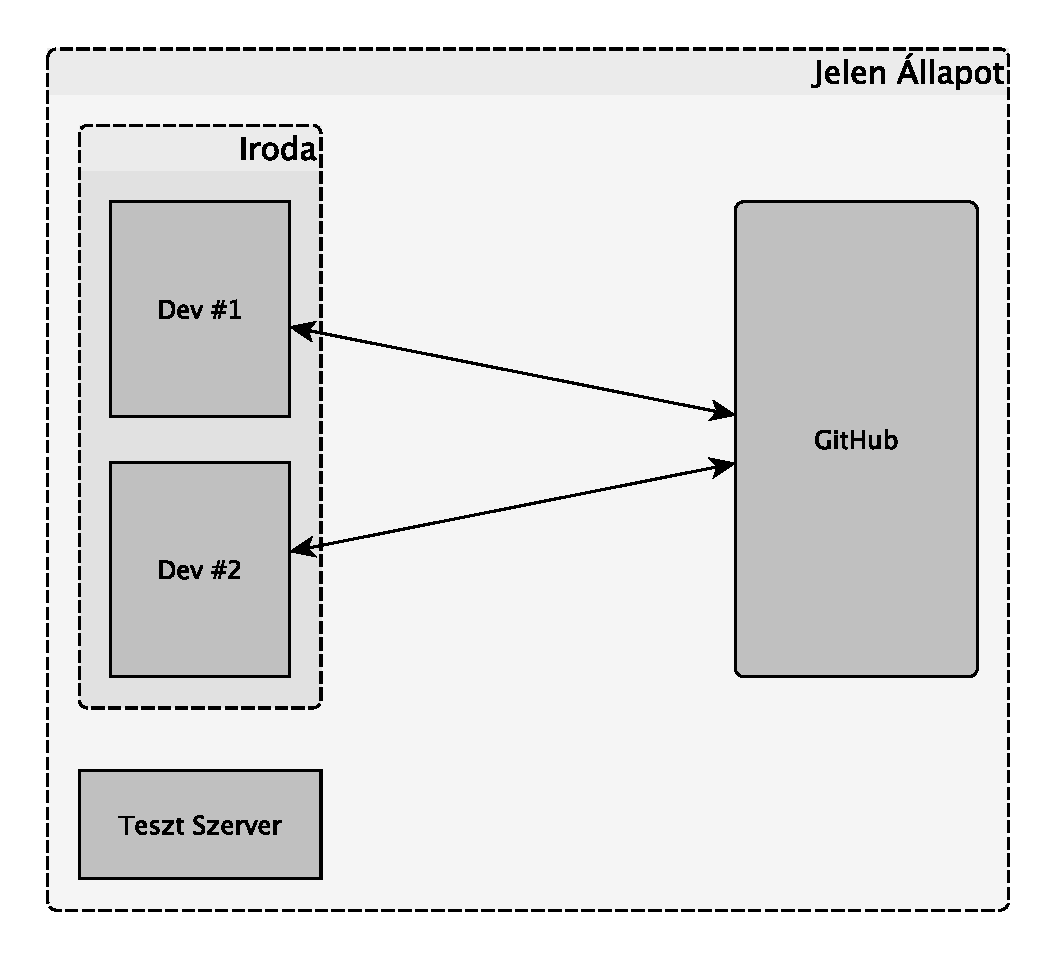
\includegraphics[width=0.7\linewidth]{figures/jelenallapot}
	\caption{Jelen Állapot}
	\label{fig:jelenallapot}
\end{figure}

Az új rendszernek a jelenlegi állapotnak több sajátosságát meg szerettem volna tartani és ezeken felül a már meglévő szerverekkel megvalósítani a rendszer működését. 
Fontosnak tartottam hogy a fejlesztők kizárólag a feladataik csökkenésével szembesüljenek és ne keljen új programokat, folyamatokat megtanulniuk 
Kvázi ne látszódjon a háttérbe folyó változás és a jelenlegi rendszer szolgáltatás kiesésével se járjon az új rendszer bevezetése. 
Mivel az ILONA fejlesztése teljesen önerőből, támogatás nélkül valósul meg, ezért törekedtem arra hogy csak ingyenes, opensource alkalmazásokat használjak a feladathoz. 
--------------
A jelenlegi rendszer alapja az egyik legnépszerűbb ingyenes internetes verziókövető rendszer a GitHub. 
A GitHub-ot feltétlen meg akartam tartani az új rendszerben mivel egy elterjedten használt és kedvelt környezetnek tartom és ami még mellette szól az az ingyenessége. 
Ez a teszt szerver Maven segítségével építi és teszteli a megírt kódokat, ezért a következő amit a meglévő rendszerből át akartam vinni az újba az a Maven. 
A jelenlegi rendszer nem hatékony a munkavégzés során, mivel számos munkaidőt emészt fel a folyamat amely nem a fejlesztéssel kapcsolatos. 
--------------
\pagebreak
\paragraph{}
A fejlesztőknek az új rendszerben lényegében csak a GitHubbal és a kész JAR fájlokat tartalmazó repository szerverrel kell dolgozniuk a többi folyamatot automatikusan látná el a rendszer. 
A cél tehát egy olyan Automatikus Tesztelési Környezet megvalósítása, amely képes a GitHubról letölteni a kódokat akkor ha a kódban változás történik. 
Ezen felűl ha a tesztek és a buildelési folyamat is sikeresen végbement az elkészült fájlokat könnyen és szervezetten elérhetővé tennie egy repository szerveren. 
Ez a tervezett folyamat látható a \ref{fig:jovoallapot} ábrán. 


\begin{figure}[h]
	\centering
	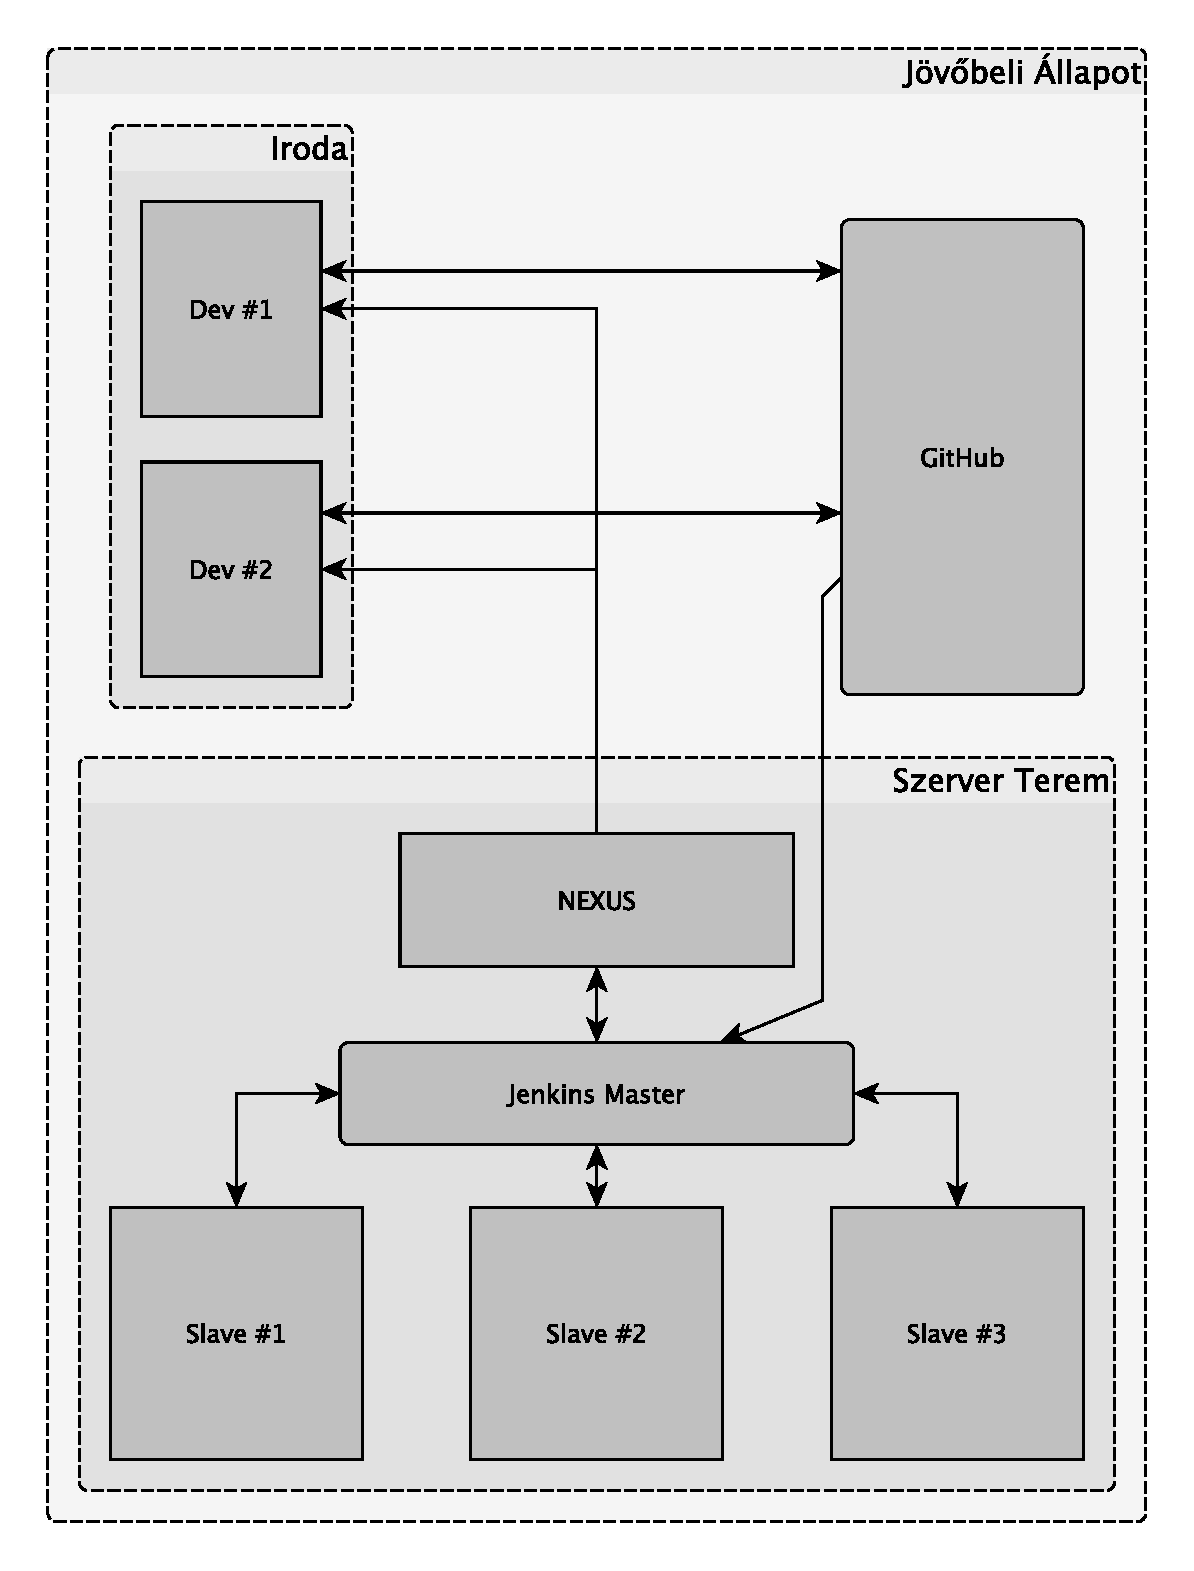
\includegraphics[width=0.7\linewidth]{figures/jovoallapot}
	\caption{Jövő Állapot}
	\label{fig:jovoallapot}
\end{figure}

--- IDE MÉG KELL ÍRNI ---
